\section{Обзор}
%\subsection{Основные определения из области формальных языков}
\subsection{Обобщённый синтаксический анализ}
Большинство языков программирования могут быть описаны однозначной КС-грамматикой, но создание такой грамматики является трудоёмким и долгим процессом. На практике, как правило, спецификацию необходимо получить быстро, по этой причине доступная для разработчиков спецификация языка часто содержит неоднозначности. Приведение грамматики к детерминированной форме --- процесс сложный, часто приводящий к появлению ошибок. Для работы с неоднозначными грамматиками используются алгоритмы обобщённого синтаксического анализа. Такие алгоритмы рассматривают все возможные пути разбора входной цепочки и строят все деревья вывода для неё.

Впервые такой подход был предложен в работе~\cite{Tomita}: на основе алгоритма восходящего синтаксического анализа LR был разработан алгоритм GLR. Такой алгоритм позволил обрабатывать конфликты типа shift/reduce и reduce/reduce, которые не могут быть корректно обработаны обычными LR-анализаторами. Принцип работы GLR-алгоритма остался таким же, как и у LR-алгоритма, но для заданной грамматики GLR-парсер строит все возможные выводы входной последовательности, используя поиск в ширину. В ячейках LR-таблиц хранится не более одного правила свёртки для текущего символа во входном потоке. В ячейках таблицы GLR-парсера может храниться несколько правил свёртки. Эта ситуация соответствует конфликту типа reduce/reduce. Когда возникает конфликт, т.е. символ на входе может быть разобран несколькими разными способами, стек парсера разветвляется на два или больше параллельных стека. Верхние состояния этих стеков соответствуют возможным переходам. Если для какого-либо верхнего состояния и входного символа в таблице не существует ни одного перехода, то эта ветка разбора считается ошибочной и отбрасывается. 

Позже было предложено множество модификаций GLR-алгоритма: RIGLR~\cite{RIGLR}, RNGLR~\cite{RNGLR}, BRNGLR~\cite{BRNGLR}. Восходящие анализаторы в отличие от нисходящих, как правило, имеют сложную структуру и трудны для разработки. В 2010 году был предложен алгоритм обобщённого анализа Generalised LL (GLL)~\cite{GLL} на основе алгоритма нисходящего синтаксического анализа. Основная идея осталась прежней --- просмотр всех возможных путей разбора и ветвление стека в случае возникновения неоднозначностей. В силу особенностей работы LL-алгоритма соответствующие анализаторы более просты для разработки, и, кроме того, они имеют более высокую скорость работы.

Прежде чем переходить к описанию процесса работы алгоритма, рассмотрим принцип работы синтаксических анализаторов, созданных с помощью метода рекурсивного спуска (Recursive Descent, RD). RD-анализаторы являются процедурной интерпретацией грамматики. Их непосредственная связь с грамматикой упрощает их разработку, отладку и внесение изменений при необходимости. Рассмотрим простую грамматику $G_0$ (листинг~\ref{grmG0}) и соответствующий анализатор, написанный методом рекурсивного спуска.

\begin{listing}
\caption{Грамматика $G_0$}
\label{grmG0}
\centering
$\begin{array}{rl}
s & \rightarrow a \ b \ | \ b \ C \\
b & \rightarrow A \ | \ C \\
a & \rightarrow A 
\end{array}$
\end{listing}

Анализатор, созданный с помощью метода рекурсивного спуска, для данной грамматики будет состоять из функций для разбора нетерминалов --- $parseS()$, $parseB()$, $parseA()$, и управляющей процессом разбора функции main(). Но поскольку данная грамматика не является однозначной, разбор даже корректного входа, например, цепочки {\it ``ac''}, будет заканчиваться ошибкой. Кроме того, в худшем случае время работы таких парсеров может экспоненциально зависеть от размера входа для сильнонеоднозначных грамматик. 

Алгоритм Generalised LL является обобщением алгоритмов LL и рекурсивного спуска и способен обрабатывать все контекстно свободные грамматики, в том числе содержащие левую рекурсию. Как и в классическом рекурсивном спуске, в GLL-анализаторах сохраняется тесная связь с грамматикой, что упрощает  реализацию и отладку. Вместе с этим, расход памяти и время работы в худшем случае является кубическим относительно размера входа и линейным для LL-грамматик. Это обеспечивается за счёт использования специализированных структур данных хранения стека и леса разбора.

\subsection{Структурированный в виде графа стек}
Стек в алгоритмах синтаксического анализа используется для того, чтобы запоминать ранее разобранные символы. Поскольку алгоритмы обобщённого синтаксического анализа строят все возможные выводы входной строки, необходимо для каждого варианта разбора хранить свой стек. Как только в процессе разбора происходит конфликт, создаётся несколько новых процессов анализа и каждый из них будет иметь свой собственный стек. Каждый такой стек будет иметь общую часть и разным у них будет только верхнее состояние. Проблема данного подхода заключается в том, что хранение отдельных стеков в явном виде требует слишком больших накладных расходов. Для того, чтобы бороться с этим, стеки комбинируются с помощью структуры данных GSS (Graph Structured Stack). В результате всё множество стеков представляется в виде графа, а в качестве вершины конкретного стека можно хранить только указатель на соответствующую вершину графа. На рис.~\ref{GSS} показан пример объединения нескольких стеков: для стеков S1, S2 и S3 в результате будет получен S1.

\begin{figure}
 \centering
 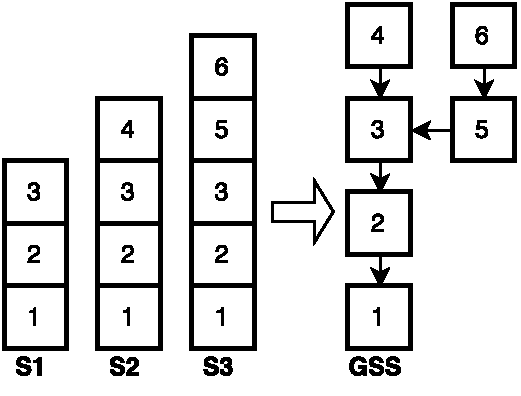
\includegraphics[width=0.6\textwidth]{Ragozina/pics/GSS.pdf}
 \caption{Стек, структурированный в виде графа  }
 \label{GSS}
\end{figure}

В вершине GSS хранится правило грамматики с указанием позиции в правой части (обозначается $X \rightarrow \alpha x \cdot \beta$, дальше просто \textit{слот}) и позиция во входном потоке. Позиция во входном потоке используется для того, чтобы различать вершины стека. На ребре GSS хранится часть леса разбора, построенное на соответствующем шаге работы анализатора. Описанное представление GSS обладает существенным недостатком: многие вершины и рёбра дублируются. Для примера рассмотрим грамматику $G_1$ (листинг~\ref{grmG1}).

\begin{listing}
\caption{Грамматика $G_1$}
\label{grmG1}
\centering
$\begin{array}{rl}
a \rightarrow A \ a \ B \ | \ A \ a \ C \ | \ A
\end{array}$

\end{listing}
Для такой грамматики в процессе разбора будет построен GSS (в дальнейшем просто стек), показанный на рис. 2({\it а}). На рисунке видно, что рёбра дублируются. Этот же стек может быть представлен как показано на рис. 2({\it б}). Таким образом можно значительно уменьшить размер графа без потери информации. 

\begin{figure}
 \centering
 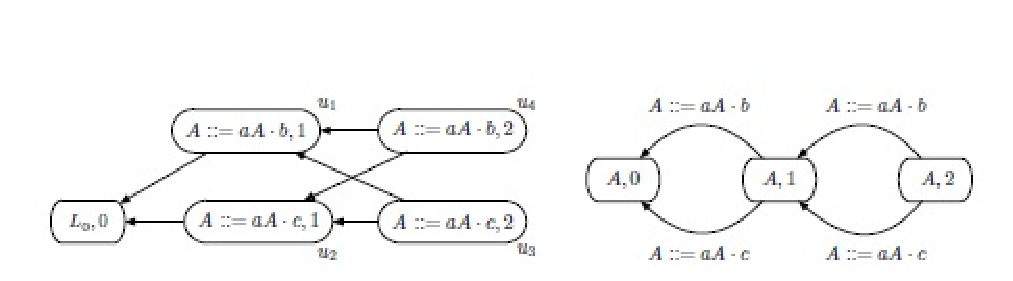
\includegraphics[width=\textwidth]{Ragozina/pics/GSSNew.pdf}
 \caption{{\it а} --- старая версия GSS;  {\it б} --- модифицированный GSS }
 \label{GSS2}
\end{figure}

Данная модификация стека предложена в работе~\cite{Afroozeh2015}, посвященной улучшению производительности работы алгоритма GLL. Уменьшение количества рёбер в стеке достигается за счёт хранения в вершинах не слота целиком, а только имени нетерминала и позиции во входном потоке. Соответствующий слот в описанном варианте хранится на ребре стека. В конечном итоге уменьшение количества вершин и рёбер позволяет значительно ускорить время работы алгоритма и уменьшить объём потребляемой памяти~\cite{Afroozeh2015}. В данной работе были использованы эти результаты.

\subsection{Сжатое представление леса разбора}
Результатом работы синтаксического анализатора является дерево разбора. Для неоднозначных грамматик для одной и той же входной цепочки может быть построено несколько различных деревьев, для некоторых грамматик количество деревьев может экспоненциально зависеть от размера входа. Для того, чтобы уменьшить количество требуемой для хранения деревьев памяти, используется структура данных Shared Packed Parse Forests (SPPF)~\cite{SPPF}, которая позволяет хранить лес разбора более компактно. Это достигается за счёт того, что в SPPF узлы с одинаковыми деревьями под ними переиспользуются, а узлы, которые соответствуют разным выводам одной и той же цепочки из одного и того же нетерминала, комбинируются. Например, для сильно неоднозначной грамматики $G_2$ (листинг~\ref{grmG2}) и входной цепочки  {\it ``bbb''} может быть построено два дерева, показанных на рис.~\ref{SPPF1}{\it (a)} и рис. ~\ref{SPPF1}{\it (б)}, которые могут быть сжаты в SPPF так, как показано на рис.~\ref{SPPF1}{\it (в)}.

\begin{listing}
\caption{Грамматика $G_2$}
\label{grmG2}
\centering
$\begin{array}{rl}
s \rightarrow s \ s \ | \ B
\end{array}$
\end{listing}

\begin{figure}
 \centering
 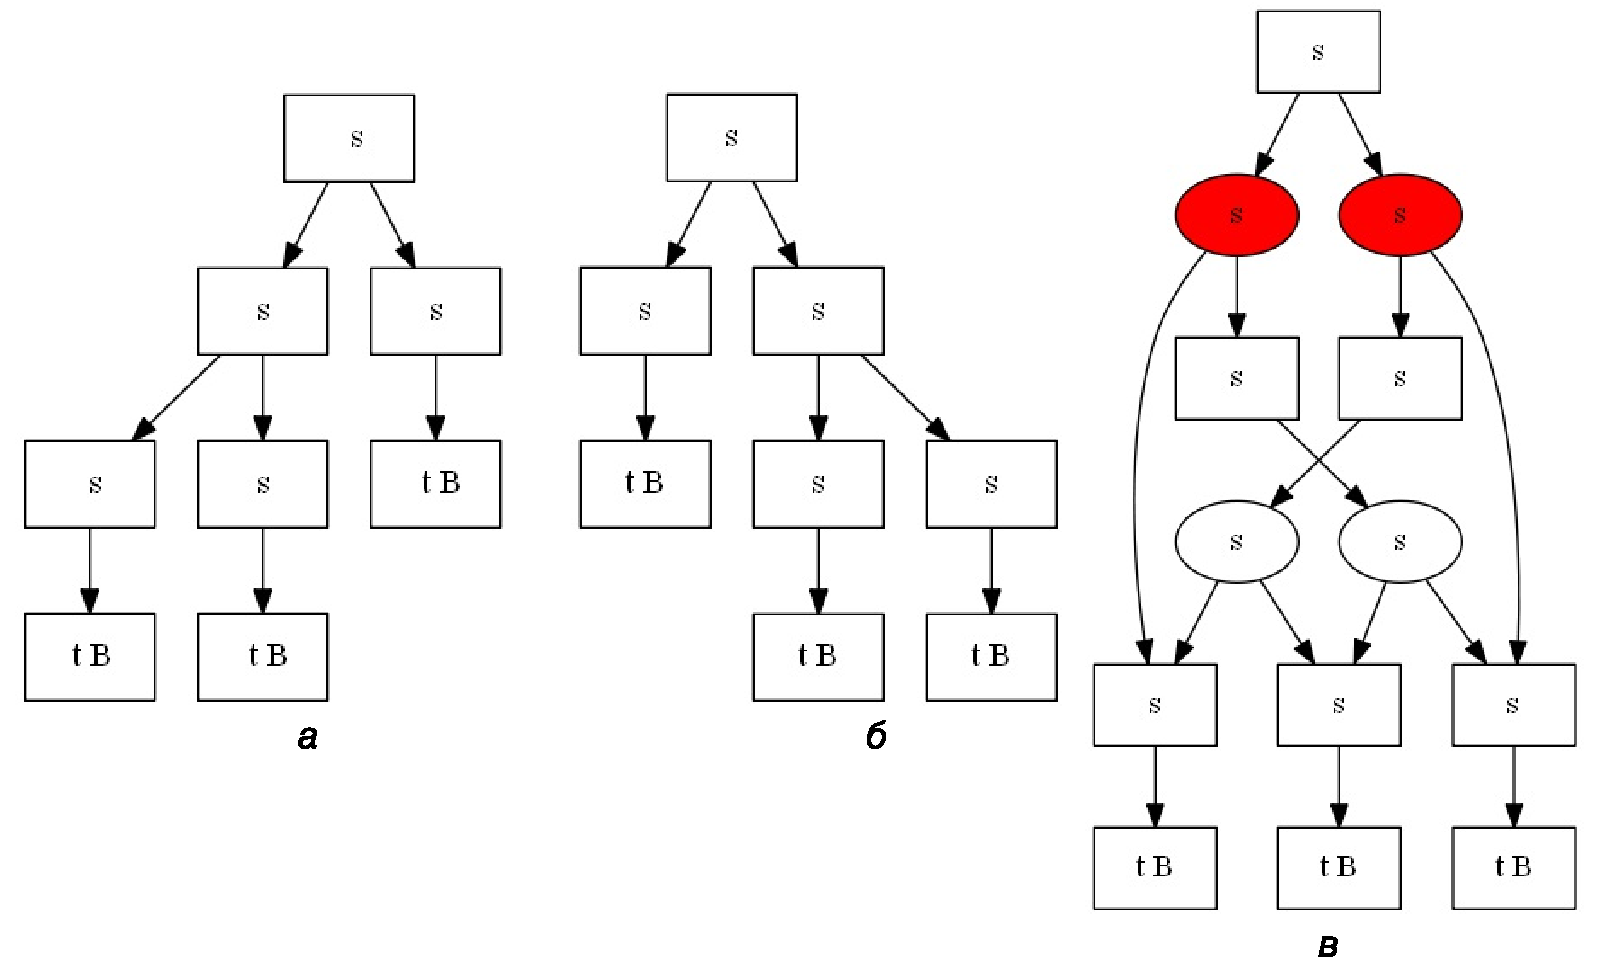
\includegraphics[width=\textwidth]{Ragozina/pics/SPPF1.pdf}
 \caption{{\it а} --- левый вывод; {\it б} --- правый вывод; {\it в} --- сжатое представление леса разбора }
 \label{SPPF1}
\end{figure}

В алгоритме GLL строится бинаризированная версия SPPF, в которой используется три типа узлов --- символьные, упакованные и промежуточные узлы. Символьные узлы представляют собой тройку $(x, i , j)$, где $х$ имя нетерминала или терминала (различают, соответственно, терминальные и нетерминальные узлы), а $i$ и $j$ --- позиции во входном потоке, которым соответствует рассматриваемая часть дерева (для корня --- узла, помеченного стартовым нетерминалом, --- начальной позицией будет 0, а конечной длина строки). Позиции во входном потоке дальше будем называть правой и левой координатами узла. Промежуточные узлы хранят слот и позиции во входном потоке. Упакованные узлы имеют вид ($ a \rightarrow \gamma \cdot, k$), где $k$ --- правая позиция для левого сына, которая используется для того, чтобы различать узлы. Терминальные узлы не имеют потомков и являются листьями в SPPF. Нетерминальные и промежуточные узлы могут иметь несколько потомков, упакованные узлы имеют только оного или двух, где правым потомком является символьный узел вида $(x, k, i)$, а левым, если существует, --- символьный или промежуточный узел вида $(s, j, k)$. Упакованные узлы используются для описания фактов неоднозначности в выводе, т.е. если у нетерминала более одного упакованного узла в потомках, то для этого нетерминала было построено несколько выводов одной и той же цепочки. На рис.~\ref{SPPF2} изображен SPPF для грамматики $G_2$.

\begin{figure}
 \centering
 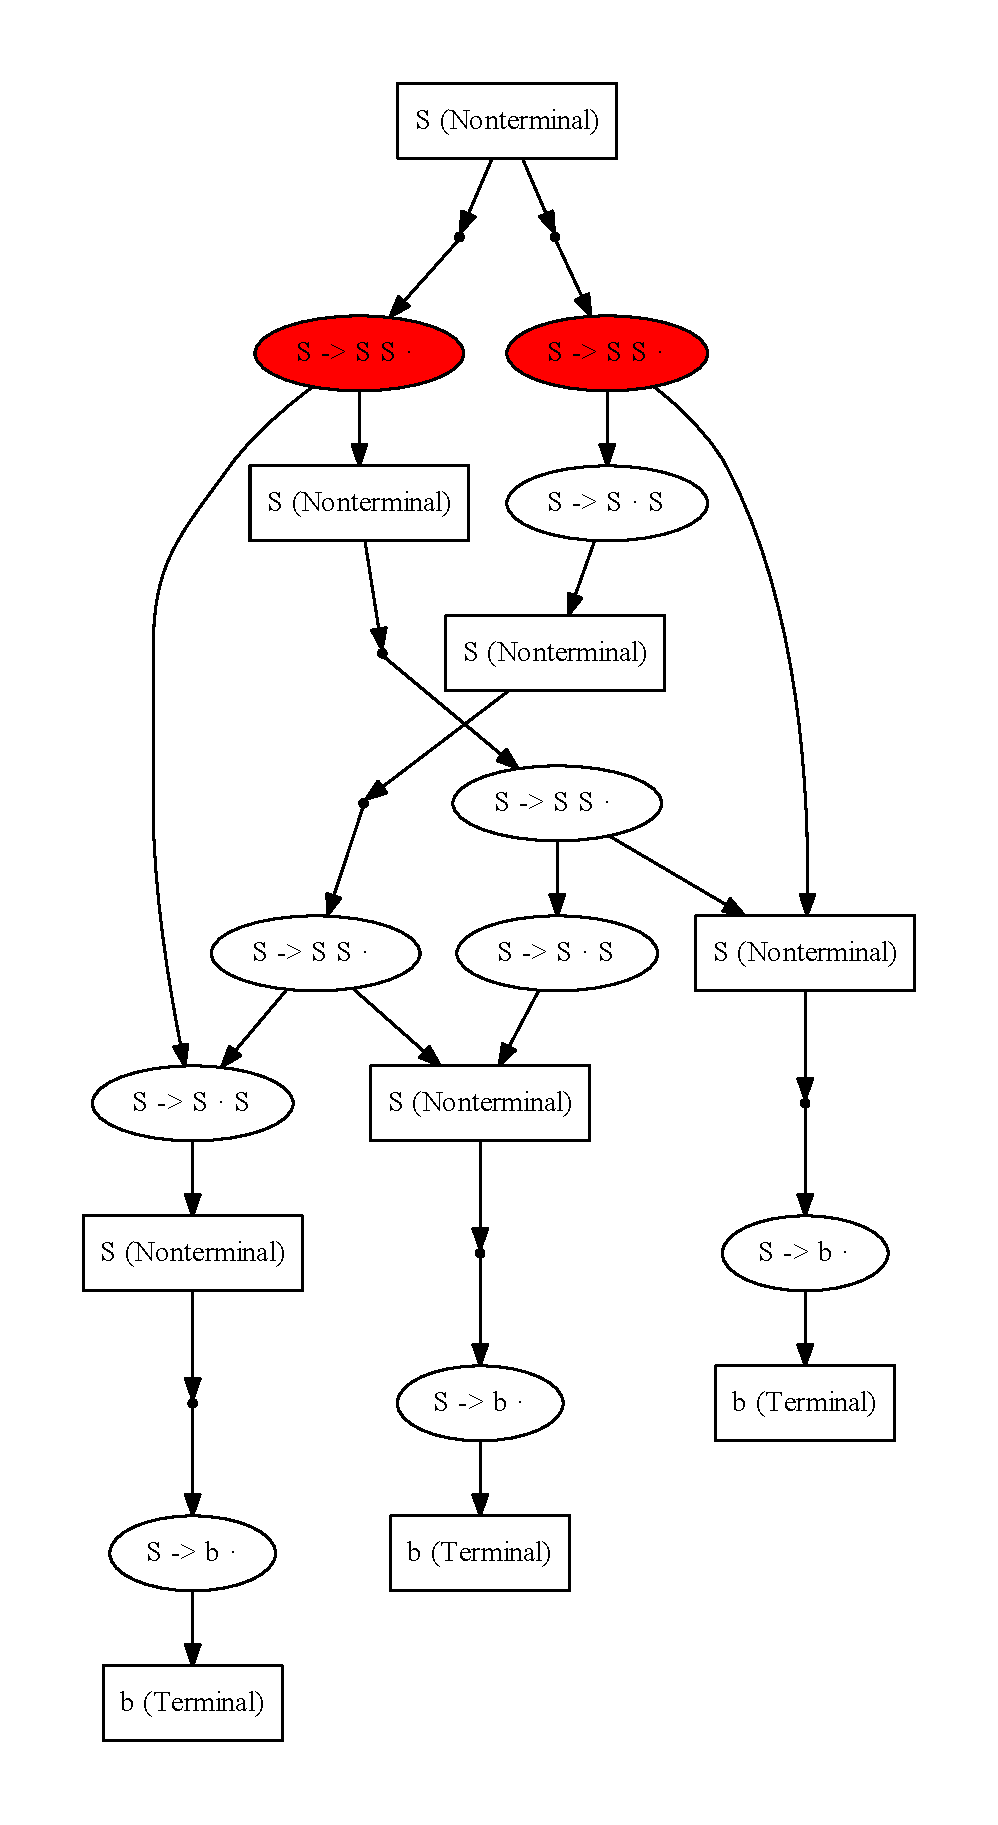
\includegraphics[width=0.8\textwidth]{Ragozina/pics/GLLSppf.pdf}
 \caption{Бинаризированное представление сжатого леса разбора для грамматики $G_2$ и входной строки {\it ``bbb''} }
 \label{SPPF2}
\end{figure}

На рис.~\ref{SPPF2} точками обозначены упакованные узлы. Узлы, помеченные слотами, являются промежуточными, а терминальные и нетерминальные узлы подписаны. У стартового нетерминала имеется два потомка, что свидетельствует о существовании двух выводов для данной входной цепочки.

\subsection{Алгоритм GLL}
Процесс работы GLL-анализатора можно рассматривать как обход грамматики в соответствии со входным потоком. На каждом шаге выполнения GLL анализатор находится в некоторой позиции в грамматике вида $x \rightarrow \alpha X \cdot \beta$, которая обозначается $L$, и поддерживает три переменные: текущая позиция во входном потоке (cI), текущая вершина стека (cU) и текущий узел в дереве (cN). Эта четвёрка называется дескриптором и позволяет полностью описать текущий шаг разбора. Дескрипторы извлекаются из очереди и разбор каждый раз начинается заново с точки, описанной в дескрипторе. Если какой-то путь не может быть продолжен, то процесс анализа не заканчивается ошибкой: вместо этого из очереди извлекается следующий дескриптор и процесс возобновляется с точки, описанной в нём. Алгоритм останавливается, как только очередь дескрипторов становится пустой.

Синтаксический анализатор состоит из набора функций с уникальными метками, управление между которыми передаётся с помощью оператора \texttt{goto()}. В отличии от парсеров, созданных с помощью метода рекурсивного спуска, в GLL-анализаторах функции генерируется для каждой альтернативы и у \texttt{goto()} может быть несколько целевых меток. Функции бывают двух видов: для каждой альтернативы нетерминала, соответствующие слотам в грамматике вида $a \rightarrow \cdot\gamma$, и функциями для слотов вида $ y \rightarrow \delta x \cdot \mu$. При создании дескриптора в качестве текущей позиции в грамматике запоминается имя целевой функции. Кроме того, имеется управляющая функция, которая извлекает очередной дескриптор из очереди и вызывает соответствующую функцию с помощью операции \texttt{goto()}. Также есть функция для построения стека \texttt{create()} и для построения дерева \texttt{getNodeP()} и \texttt{getNodeT()}. Функция \texttt{getNodeT()} используется для создания терминального узла, а \texttt{getNodeP()} для создания всех остальных видов узлов.

Стек частично заменяет вызов функции в парсерах, написанных методом рекурсивного спуска. Вершины стека создаются, как только в процессе обхода грамматики встречается нетерминал (например, $x \rightarrow \alpha \cdot a \beta$). Как упоминалось ранее, на вершинах стека находятся пары $(N, i)$, где $N$ --- имя нетерминала, который необходимо разобрать, $i$ --- позиция во входном потоке на момент создания вершины. На ребре хранится слот и часть леса разбора. Слот позволяет сохранить информацию о том, в какую позицию в грамматике необходимо вернуться после того, как нетерминал будет разобран (в случае слота $x \rightarrow \alpha a \cdot \beta$ разбирается нетерминал a). Второй элемент пары --- часть леса разбора, которая была построена на момент создания вершины стека (для рассматриваемого слота $x \rightarrow \alpha a \cdot \beta$ это часть SPPF для цепочки $\alpha$). После того, как нетерминал будет разобран, вершина извлекается из стека и для всех исходящих рёбер создаются новые дескрипторы $(l, i, u, t)$, где $l$ --- слот с ребра, $i$ --- текущая позиция во входном потоке, $u$ --- целевая вершина ребра и $t$ --- часть леса разбора, полученная объединением части леса с ребра и построенной для нетерминала (для рассматриваемого слота $x \rightarrow \alpha a \cdot \beta$ объединяется часть леса для цепочки $\alpha$ и нетерминала $A$).

\begin{listing}
\caption{Грамматика $G_3$}
\label{grmG3}
\centering
$\begin{array}{rl}
s \rightarrow A \ s \ B \ | \ D \ | \ A \ D \ B 
\end{array}$
\end{listing}

Кроме того, для корректной работы алгоритма используются дополнительные множества. Все дескрипторы добавляются в очередь $R$ и последовательно извлекаются из неё в процессе работы анализатора. Процесс работы синтаксического анализатора недетерминирован и может возникнуть ситуация, когда один и тот же дескриптор будет создаваться снова и снова. Повторное создание дескриптора приводит к тому, что процесс зациклится и никогда не завершится. Для того, чтобы избежать дублирования дескрипторов, отдельно хранится множество $U$ ранее созданных дескрипторов. В очередь добавляются только дескрипторы, не содержащиеся во множестве $U$. Для того, чтобы хранить и переиспользовать уже разобранные нетерминалы используется множество $P$. В нём хранятся пары вида $(u; z)$, где $z$ --- узел SPPF, а $u$ --- вершина GSS. Ниже приведён пример GLL-анализатора для грамматики $G_3$. В приведённом примере функция $L_0$ содержит основной цикл, который извлекает дескрипторы из очереди и присваивает переменным cU, cI  и cN значения из извлечённого дескриптора. 

\begin{figure}
 \centering
 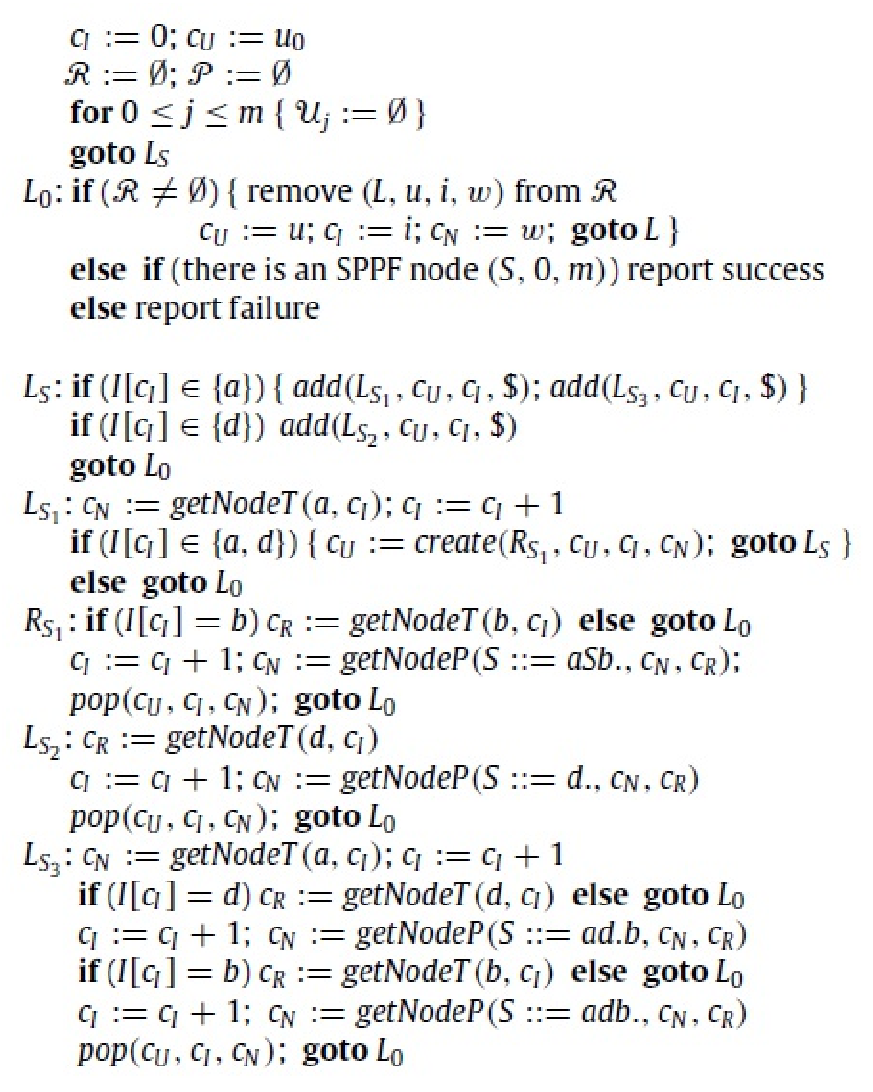
\includegraphics[width=\textwidth]{Ragozina/pics/Listing1.pdf}
 \label{ListingGLL1}
 \caption{GLL-анализатор для грамматики $G_3$ }
\end{figure}

\subsection{Подходы к анализу встроенных языков}
В области анализа встроенных языков ведутся исследования и разрабатываются инструменты, реализующие различные подходы. 
\begin{itemize}
\item Java String Analyzer (JSA)~\cite{JSA,JSAUrl} --- инструмент для анализа строк и строковых операций в программах на Java. Основан на проверке включения регулярной аппроксимации встроенного языка в контекстно-свободное описание эталонного языка.
\item PHP String Analyzer (PHPSA)~\cite{PHPSA,PHPSAUrl} --- инструмент для статического анализа строк в программах на PHP. Расширяет подход инструмента JSA. В инструменте уточнена проводимая аппроксимация и это повышает точность проводимого анализа. 
\item Alvor~\cite{AlvorUrl, Alvor2, Alvor1} --- плагин к среде разработки Eclipse, предназначенный для статической проверки корректности SQL-выражений, встроенных в Java. Для компактного представления множества динамически формируемого строкового выражения используется понятие абстрактной строки, которая, фактически, является регулярным выражением над используемыми в строке символами. В инструменте Alvor отдельным этапом выделен лексический анализ. Поскольку абстрактную строку можно преобразовать в конечный автомат, то лексический анализ заключается в преобразовании этого конечного автомата в конечный автомат над терминалами при использовании конечного преобразователя, полученного генератором лексических анализаторов JFlex. Несмотря на то, что абстрактная строка позволяет описывать строковые выражения при конструировании которых использовались циклы, плагин в процессе работы выводит сообщение о том, что данная языковая конструкция не поддерживается. Также инструмент Alvor не поддерживает обработку строковых операций, за исключением конкатенации, о чём также выводится сообщение во время работы.
\item IntelliLang~\cite{IntelliLang} --- плагин к средам разработки IntelliJ IDEA и PHPStorm, предоставляющий поддержку встроенных строковых языков, таких как HTML, SQL, XML, JavaScript в указанных средах разработки. Данное расширение обеспечивает подсветку синтаксиса, автодополнение, статический поиск ошибок. Для среды разработки IntelliJ IDEA расширение IntelliLang также предоставляет отдельный текстовый редактор для работы со встроенным языком. Для использования данного плагина требуется ручная разметка переменных, содержащих выражения на том или ином встроенном языке.
\item Varis~\cite{Varis} --- плагин для Eclipse, представленный в 2015 году и предоставляющий поддержку кода на HTML, CSS и JavaScript, встроенного в PHP. В плагине реализованы функции подсветки встроенного кода, автодополнения, перехода к объявлению (jump to declaration), построения графа вызовов (call graph) для встроенного JavaScript. 
\end{itemize}

Все эти инструменты предназначены для решения достаточно узких задач и часто не предусматривают проведения сложного анализа динамически формируемого кода. Более сложные виды анализа могут быть произведены с применением абстрактного синтаксического анализа, который предложен в работе~\cite{LrAbstract2}. Алгоритм абстрактного синтаксического анализа комбинирует анализ потока данных и синтаксический LR-анализа. Входными данными для него является набор data-flow уравнений, описывающих множество значений динамически формируемого кода. Данные уравнения решаются в домене LR-стеков при помощи абстрактной интерпретации~\cite{AbstractInterpretation}, обеспечивающей свойство завершаемости алгоритма. Результатом работы является набор абстрактных синтаксических деревьев, которые в дальнейшем могут использоваться для решения различных задач статического анализа. К сожалению, в работах отсутствует рассмотрение эффективного представление результатов анализа. Кроме того, инструментов, реализующих предложенный подход, в открытом доступе нет.

Также существует подход к обработке динамически формируемого кода,  основанный на алгоритме обобщённого восходящего анализа RNGLR~\cite{RelaxedARNGLR}. Подход основан на проверке включения регулярного языка в некоторые подклассы КС-языков. В качестве входных данных в работе используется регулярное приближение множества всех значений динамически формируемого кода в некоторой точке программы-генератора. Данное приближение описывается регулярным языком $L$ и является приближением сверху (over-approximation) для множества возможных значений: регулярный язык содержит все предложения, генерируемые программой и, возможно, ещё какие-то. Благодаря этому можно говорить о достоверности многих видов статического анализа. Таким образом, регулярная аппроксимация для множества значений динамически формируемых выражений позволяет решать многие важные задачи, например, поиск ошибок во встроенном коде. Для представления регулярной аппроксимации используются конечные автоматы, так как для любого регулярного языка $L$ можно построить конечный автомат, такой что он принимает те и только те цепочки, которые принадлежат языку $L$. Далее построенный конечный автомат подаётся на вход лексическому анализу (преобразуется из автомата над символами в автомат над токенами), а затем синтаксическому анализу, алгоритм которого основан на алгоритме RNGLR. Достоинствами предложенного решения являются модульность, позволяющая рассматривать различные этапы анализа отдельно, и возможность построения конечного леса вывода для всех корректных цепочек из $L$, что позволяет реализовывать различные виды анализа динамически формируемого кода, требующие его структурного представления.

\subsection{YaccConstructor}
YaccConstructor~\cite{YCUrl} --- исследовательский проект лаборатории языковых инструментов JetBrains, направленный на изучение алгоритмов лексического и синтаксического анализа. Проект включает в себя одноимённый модульный инструмент с открытым исходным кодом, предоставляющий платформу для разработки лексических и синтаксических анализаторов, содержащую большое количество готовых компонент, таких как различные преобразования грамматик, язык описания атрибутных грамматик YARD и др. Большинство компонент реализованы на платформе .NET, основным языком разработки является F\# ~\cite{FSharp}. Предоставляемый язык спецификации грамматик YARD, поддерживает атрибутные грамматики, грамматики в расширенной форме Бэкуса-Наура и многое другое.

В рамках проекта была создана платформа для статического анализа динамически формируемого кода, основанная на модульной архитектуре, предложенной в~\cite{GrigorievPhd}. В рамках соответствующих модулей реализованы механизмы лексического анализа, описанный в~\cite{polubelova}, и алгоритм синтаксического анализа, описанный в~\cite{RelaxedARNGLR}. Благодаря модульной архитектуре, данные компоненты могут использоваться независимо. 

\subsection{Анализ метагеномной сборки}
В биологических исследованиях часто необходимо ответить на вопрос, к какому виду относится тот или иной организм. Образцы часто берутся из окружающей среды и могут быть не идентифицированы. По таким образцам строится метагеномная сборка, являющаяся множеством участков ДНК различных организмов. Такое множество может быть представлено в виде конечного автомата, порождающего геномы всех организмов, содержащихся в образце. Саму последовательность ДНК можно рассматривать, как строку в алфавите $\{A, C, G, T\}$, однозначно определяющую организм (или штамм), к которому она относится. 

Наиболее часто используемый подход для идентификации образцов, взятых из окружающей среды, --- проведение сравнительного анализа последовательности рРНК. Поскольку большая часть информации об организме хранится именно в рРНК. При этом для поиска и идентификации подцепочек используется несколько основных механизмов: скрытые цепи Маркова, используемые в таких инструментах, как HMMER~\cite{hmmer}, REAGO~\cite{reago}, ковариационые модели (covariation model, CM)~\cite{durbin}, основанные на вероятностных грамматиках и применении синтаксического анализа для задачи поиска. Однако проблема заключается в том, что восстановление небольших участков рРНК по объёмной метагеномной сборке оказывается трудоёмким и не всегда её может быть решена эффективно. 

Существующие подходы для решения такой задачи можно разделить на два класса. Первый класс сначала использует инструменты для анализа сборок de novo (полные геномные последовательности организмов, находящихся в метагеномной сборке, ещё не известны), которые восстанавливают геномные последовательности в линейном виде. Затем результат их работы передаётся инструментам геномного поиска рРНК. Проблема данных инструментов заключается в том, что восстановление генов в метагеномной сборке задача очень трудоёмкая. Кроме того, большая часть генов de novo состоит из участков, не носящих информации о рРНК. Таким образом, подход построения метагеномой сборки и поиска рРНК по ней с использованием сторонних инструментов не оптимален. 

Другой класс инструментов реализует поиск непосредственно в метагеномной сборке. Часть из них используют предварительную фильтрацию отдельных линейных участков (предполагается, что сборка ещё не представлена в виде конечного автомата), что позволяет избавиться от анализа последовательностей, не несущих необходимой информации. Затем из оставшихся частей производится сборка pРНК. Такой подход используется в EMIRGE~\cite{Emirge}. Недостатком подхода является необходимость наличия большого числа известных рРНК и высокая вероятность не найти далеко стоящие друг от друга рРНК. Инструмент REAGO лишён этих проблем, однако он не работает с метагеномной сборкой, представленной в виде графа, а хранение сборки в виде набора прочитанных участков требует большого объёма памяти.

Обработка сборки, представленной в виде графа реализована в инструменте Xander~\cite{Wang2015}, который использует для решения задачи композицию скрытых моделей Маркова (HMM) и входного графа. Недостатком такого подхода является то, что использование HMM даёт существенно более низкую точность результата по сравнению с использованием CM~\cite{EddyComputationalRNA}. Наиболее известным инструментом, использующим CM для поиска рРНК является Infernal~\cite{Infernal}. Однако он не применим к метагеномным сборкам, представленным в виде графа.

\subsection{Выводы}
В результате выполненного обзора были сделаны следующие выводы.
\begin{enumerate}
\item Алгоритм синтаксического анализа, предложенный в работе~\cite{RelaxedARNGLR} позволяет решать задачу построения леса вывода для динамически формируемого кода. Поэтому идеи, предложенные в этих работах взяты за основу данной диссертации.
\item Алгоритм синтаксического анализа GLL имеет более очевидную связь с грамматикой, чем восходящие алгоритмы анализа, поддерживает произвольные КС-грамматики и обладает высокой производительностью, что позволяет использовать его для задач синтаксического анализа регулярных множеств.
\item YaccConstructor содержит готовое решение для синтаксического анализа динамически формируемого кода, основанное на RNGL-алгоритме. При этом архитектура этого решения позволяет легко заменять алгоритмы синтаксического анализа, оставляя без изменений другие компоненты, такие как лексический анализ, построение аппроксимации~\cite{SELforIDE}. Таким образом YaccConstructor является подходящей платформой для практической реализации.
\item Применение механизмов синтаксического анализа к конечным автоматам является важной задачей в биоинформатике.
\end{enumerate}
